\chapter{Outlook}
\label{chap:outlook}

The goal of this thesis is to apply the abstract process theoretic framework for dagger symmetric monoidal categories to quantum algorithms and protocols.  In the preceding chapters, we have presented results that leverage the structure of process theories to make the following original contributions:
\begin{enumerate}
\item In Section~\ref{sec:strcomplFT}, we used strong complementarity to construct the abelian Fourier Transform over finite groups in arbitrary $\dagger$-SMCs. This indicates that it is the presence of strongly complementary observables in quantum theory that makes the Fourier Transform algorithm structurally native to quantum computation.

\item In Section~\ref{sec:blackbox}, we connect unitary oracles to complementary observables in arbitrary process theories. We then use these unitary oracles to construct a quantum algorithm for a new blackbox problem GROUPHOMID, and investigated its query complexity bounds.

\item In Section~\ref{sec:qalgrel}, an operational process theory in \cat{Rel} is used to build models of the Deutsch-Jozsa, single-shot Grover's, and GROUPHOMID quantum blackbox algorithms in the sets and relations of non-deterministic classical computation.

\item In Chapter~\ref{chap:mermin}, we characterize necessary and sufficient conditions for the Mermin locality (and Mermin non-locality) of an arbitrary operational process theory. These results answer open questions regarding the connection between phase groups and non-locality. Further, we extend this framework to present experimental tests of Mermin non-locality for any number of parties with access to an arbitrary number of measurements on systems of any size. We indicate some applications of these setups in quantum secret sharing.

\item Lastly, in Chapter~\ref{chap:qDisCo}, we use the shared process theoretic structure of natural language processing and quantum information to adapt a general quantum machine learning algorithm into a domain specific sentence classification algorithm while maintaining a quantum speedup.
\end{enumerate}

We conclude with a brief discussion of this work's future outlook.

\section{Blackbox algorithms}

Besides those already considered in this text, there are a slew of other algebraic blackbox problems for which there there are known superpolynomial speedups. These are all amenable to study using our process theoretic framework. Such work would further clarify the relationship between these algorithms as well as open new avenues for generalization and combination.

In particular the hidden shift problem and hidden non-linear structure problems as described in~\cite{childs2010quantum} look like promising places to start. In the hidden shift problem (HSP) we are presented a (not necessarily abelian) group $G$ along with two injective functions $f_0:G\to S$ and $f_1:G\to S$ for some set $S$ with the promise that
\begin{equation}
f_0(g) = f_1(sg) \qquad \mbox{ for some }s\in G.
\end{equation}
We are then tasked to find the hidden $s$. This problem is already known to be related to the hidden subgroup problem in several ways: (i) for abelian $G$, then it is equivalent to the HSP\footnote{Take the hidden subgroup problem for $G\rtimes_{\phi}\mathbb{Z}/2\mathbb{Z}$ where the homomorphism $\phi:\mathbb{Z}/2\mathbb{Z}\to$ Aut$(G)$ is given by $\phi(0)(x)= x$ and $\phi(1)(x)=x^{-1}$.} (ii) for non-abelian $G$ it is related to a HSP over a wreath product group and, when $G$ is a symmetric group, is equivalent to testing the isomorphism of rigid graphs~\cite{childs2010quantum}. A polynomial time algorithm for the abelian hidden shift problem is not known, but there is a quantum speedup from $2^{\mathcal{O}(\log |G|)}$ to $2^{\mathcal{O}(\sqrt{\log |G|)}}$ that can be achieved using the Kuperberg sieve~\cite{childs2010quantum,kuperberg2005subexponential}.

Within our oPT framework, we can easily represent the promise on the oracle. Let $\mathbb{G}$ be a system with an internal group of strongly complementary classical structures $\scpair$ where $\ket{s}$ is a classical state of $\dotonly{blackdot}$. Let $S$ be another system with a classical structure $\dotonly{graydot}$. The functions $f_0,f_1$ are then self-conjugate comonoid homomorphisms $\mathbb{G}\to S$ promised to obey:
\begin{equation}
\begin{pic}
\node [morphism] (3) at (0,0) {$f_0$};
\draw (0,-1.5) to (3.south) ;
\draw (3.north) to (0,1.5);
\end{pic}
\;=\;
\begin{pic}[scale=0.75]
                \node [style=state] (0) at (1, -1) {$s$};
                \node [style=whitedot] (1) at (0, -0) {};
                \node [style=morphism] (2) at (0, 1) {$f_1$};
                \node (3) at (0, 2) {};
                \node (4) at (-1, -1) {};
                \node (5) at (-1, -2) {};
                \draw [bend left=45, looseness=1.00] (4.center) to (1);
                \draw (1) to (2.south);
                \draw (2.north) to (3.center);
                \draw [bend left=45, looseness=1.00] (1) to (0);
                \draw (4.center) to (5.center);
\end{pic}
\end{equation}
where $\tinymult[whitedot]$ is the group multiplication in $G$. This promise specification could be used to further analyze the known quantum hidden shift algorithms as well as propose further generalizations beyond the $M$-generalized hidden shift problems of~\cite{childs2010quantum}. In that paper Childs and van Dam emphasize that little is known about the non-abelian hidden shift problem in general and that is may serve as a slightly easier version of the graph isomorphism problem in the case of symmetric groups. All of these facts make the hidden shift problem an attractive next step for process theoretic analysis, though there are competing candidates.

\section{Complexity and Categories}

Here we will propose directions for connecting the categorical reasoning used for verification of quantum algorithms to analyses of their complexity. In this thesis our analyses were limited in several ways: 
\begin{enumerate}
\item[(i)] We were limited to query complexity analyses where we could manually count the number of query calls in a diagram. 
\item[(ii)] We were limited to an analysis of deterministic protocols and lack a categorified notion of bounded error protocols. This limitation occurred both in our analysis of algorithms and in our analysis of non-locality protocols. Ideally we would have a notion of bounded error success internal to process theories.
\item[(iii)] In many ways because of the first issue, we are unable to directly connect the structure of process theories to the complexity class of problems that their processes can solve. This sort of result would be analogous to the connect between strongly complementary observables and Mermin non-locality tests from Chapter~\ref{chap:mermin}. At present we can only show what process theoretic structures enable particular \emph{implementations} of algorithms as is done in Chapter~\ref{chap:qalg}. We would prefer that complexity classes which are efficiently accessible from different  process theories should be directly related to their categorical structure.
\end{enumerate}

While these are fundamental issues, the perspective given in this thesis gives a foothold from which to begin addressing these important problems. One interesting avenue of approach would be to introduce some notion of repeatability and scaling into the diagrams of a process theory. In~\cite{kissinger2012pictures,kissinger2015tensors} a notion of !-boxes (pronounced bang boxes) was introduced formalize the intuitive notion of the $...$ that often appears in our morphisms definitions. These !-boxes appear as (sometime colored) boxes around elements of a diagram that can be arbitrarily repeated as in the following example:
\begin{equation}
\begin{pic}[scale=0.8]
                \node (0) at (0, 1.25) {};
                \node [style=whitedot] (1) at (0, 0) {};
                \node (2) at (0, -1.25) {};
                \node (3) at (-0.5, -1.75) {};
                \node (4) at (-0.5, 0.75) {};
                \node [fill=blue, label=B] (5) at (-0.5, -0.75) {};
                \node (6) at (0.5, -0.75) {};
                \node [fill=blue, label=A] (7) at (-0.5, 1.75) {};
                \node (8) at (0.5, -1.75) {};
                \node (9) at (0.5, 0.75) {};
                \node (10) at (0.5, 1.75) {};
                \draw [blue] (7) to (4.center);
                \draw [blue] (4.center) to (9.center);
                \draw [blue] (9.center) to (10.center);
                \draw [blue] (10.center) to (7);
                \draw [blue] (5) to (3.center);
                \draw [blue] (3.center) to (8.center);
                \draw [blue] (8.center) to (6.center);
                \draw [blue] (6.center) to (5);
                \draw [arrow=1] (2) to (1);
                \draw [arrow=1] (1) to (0);
\end{pic}

\;=\;\;
\left\{ \begin{pic}[xscale=0.7, yscale=0.9]
                \node [style=wire] (0) at (2, 1.25) {};
                \node [style=whitedot] (1) at (2, 0) {};
                \node [style=wire] (2) at (2, -1.25) {};
                \node [style=whitedot] (3) at (-5.75, 0) {};
                \node [style=wire] (4) at (-4, 1.25) {};
                \node [style=whitedot] (5) at (-4, 0) {};
                \node [style=wire] (6) at (-0.75, 1.25) {};
                \node [style=wire] (7) at (0.25, 1.25) {};
                \node [style=whitedot] (8) at (-0.25, 0) {};
                \node [style=wire] (9) at (6.5, 1.25) {};
                \node [style=whitedot] (10) at (6.5, 0) {};
                \node [style=wire] (11) at (7.25, 1.25) {};
                \node [style=wire] (12) at (5.75, 1.25) {};
                \node (13) at (-5, -0.25) {,};
                \node (14) at (-3.25, -0.25) {,};
                \node (15) at (0.75, -0.25) {,};
                \node (16) at (3, -0.25) {,};
                \node (17) at (8.5, 0) {$\cdots$};
                \node (18) at (7.5, -0.25) {,};
                \node (19) at (-1.25, -0.25) {,};
                \node [style=whitedot] (20) at (-2.25, 0) {};
                \node [style=wire] (21) at (-2.25, -1.25) {};
                \node [style=wire] (22) at (4.75, -1.25) {};
                \node (23) at (5.25, -0.25) {,};
                \node [style=whitedot] (24) at (4.25, 0) {};
                \node [style=wire] (25) at (3.75, -1.25) {};
                \draw [arrow=1] (2) to (1);
                \draw [arrow=1] (1) to (0);
                \draw [arrow=1] (5) to (4);
                \draw [arrow=1] (8) to (6);
                \draw [arrow=1] (8) to (7);
                \draw [arrow=1] (10) to (11);
                \draw [arrow=1] (10) to (12);
                \draw [arrow=1] (10) to (9);
                \draw [arrow=1] (21) to (20);
                \draw [arrow=1] (22) to (24);
                \draw [arrow=1] (25) to (24);
\end{pic}
 \right\}
\end{equation}
We could imagine labelled !-boxes with different asymptotic scalings and their own set of rewrite rules, e.g.:
\begin{equation}
\begin{pic}[scale=0.8]
                \node (0) at (0, 1.25) {};
                \node [style=whitedot] (1) at (0, 0) {};
                \node (2) at (0, -1.25) {};
                \node (3) at (-1.5, -1.5) {};
                \node (4) at (-0.5, 0.75) {};
                \node [fill=blue, label={$\mathcal{O}(n)$}] (5) at (-1.5, 3) {};
                \node (6) at (1.5, 3) {};
                \node [fill=blue, label={$\mathcal{O}(n)$}] (7) at (-0.5, 1.75) {};
                \node (8) at (1.5, -1.5) {};
                \node (9) at (0.5, 0.75) {};
                \node (10) at (0.5, 1.75) {};
                \draw [blue] (7) to (4.center);
                \draw [blue] (4.center) to (9.center);
                \draw [blue] (9.center) to (10.center);
                \draw [blue] (10.center) to (7);
                \draw [blue] (5) to (3.center);
                \draw [blue] (3.center) to (8.center);
                \draw [blue] (8.center) to (6.center);
                \draw [blue] (6.center) to (5);
                \draw [arrow=1] (2) to (1);
                \draw [arrow=1] (1) to (0);
\end{pic}

\;=\;
\begin{pic}[scale=0.8]
                \node (0) at (0, 1.25) {};
                \node [style=whitedot] (1) at (0, 0) {};
                \node (2) at (0, -1.25) {};
                \node (3) at (-1.5, -1.5) {};
                \node (4) at (-0.5, 0.75) {};
                \node [fill=blue, label={$\mathcal{O}(n^2)$}] (5) at (-1.5, 2.75) {};
                \node (6) at (1.5, 2.75) {};
                \node (8) at (1.5, -1.5) {};
                \node (9) at (0.5, 0.75) {};
                \node (10) at (0.5, 1.75) {};
                \draw [blue] (5) to (3.center);
                \draw [blue] (3.center) to (8.center);
                \draw [blue] (8.center) to (6.center);
                \draw [blue] (6.center) to (5);
                \draw [arrow=1] (2) to (1);
                \draw [arrow=1] (1) to (0);
\end{pic}

\end{equation}
Another way of thinking of these scaling labels is as an enrichment of a process theory in some suitably defined \emph{category of asymptotic scalings}. A process theory enriched in this way could then be related to categories of programs and algorithms as presented, for example, in~\cite{yanofsky2010towards}. Such an approach would begin to address the first and third limitations described in this section. Further, another perspective on enrichment would allow the labelling of processes with their success probability, addressing the second limitation. While these are still speculative ideas, we hope this indicates that there are many different and concrete directions to expand process theoretic analysis of algorithms in general. This structural perspective adds to the investigation of the many open questions regarding the complexity class separations of different theories.

\section{Quantum Programming Languages}

The development of more powerful quantum programming languages will allow us to better control and apply rapidly developing quantum hardware. Prominent examples of current quantum programming languages such as Quipper~\cite{green2013quipper} and LIQU$|\rangle$~\cite{wecker2014liqui} are based on the quantum circuit model. While this structural simplicity is useful initially, it quickly becomes unwieldy for complex quantum algorithms in for both the users and the hardware. For users this situation is analogous to classical programming using only boolean circuits and so clearly inefficient. Secondly, limitations in the first generation of classical control hardware for quantum processors make it advantageous to avoid having to load an entire fault-tolerant compiled circuit all at once. If we can dynamically compile to quantum circuits from higher level concepts, then we can have access to larger algorithms. A first example of this comes from reversible computation, where methods can be ``uncomputed"~\cite{yokoyama2008principles}. This would allow the loading of some circuit to implement the unitary $U$, along with a command to then run $U^{\dagger}$ that doesn't require an explicit circuit representation of $U^{\dagger}$ in advance. The control flow of these kinds of languages is can be completely represented in structured reversible flow circuits~\cite{yokoyama2008reversible}, e.g. Figure~\ref{fig:reversible}.

\begin{figure}[ht]
\centering
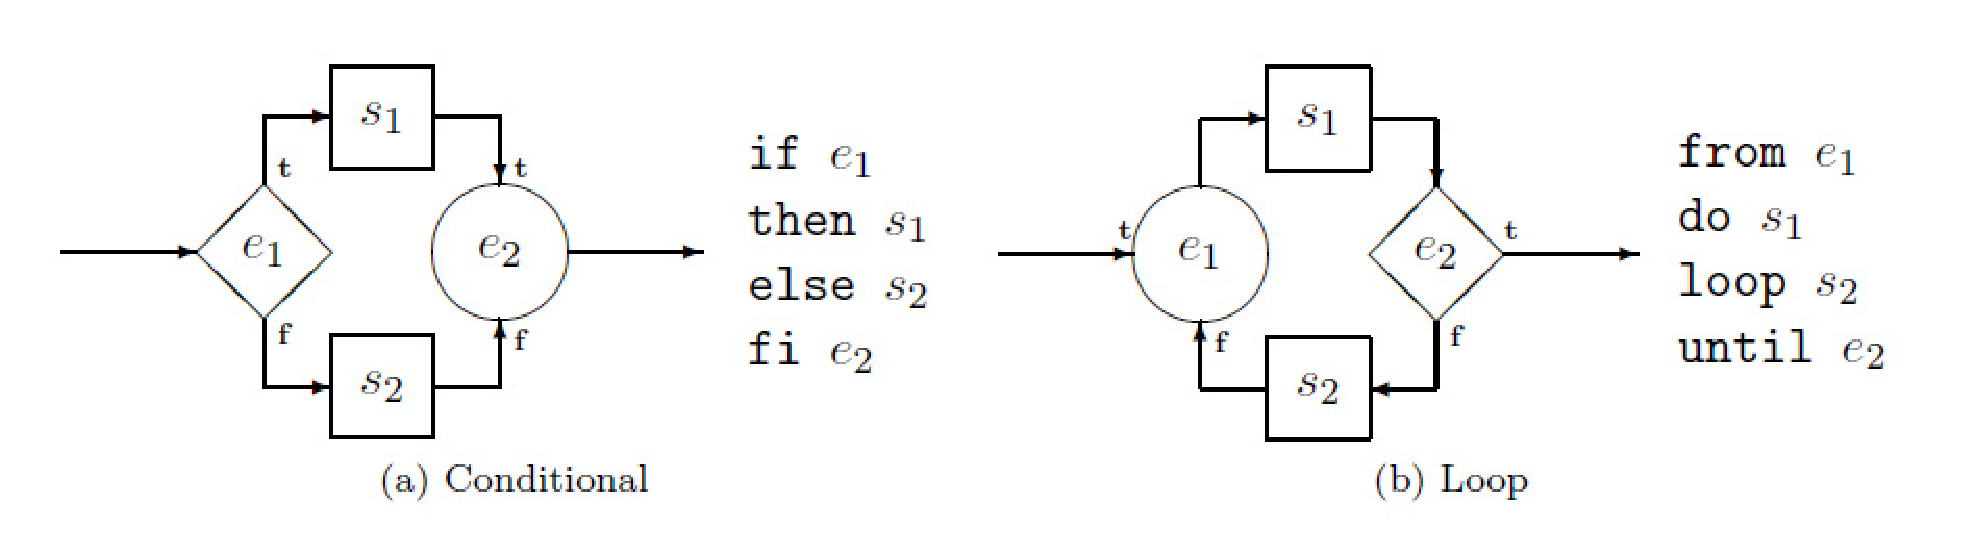
\includegraphics[scale=0.45]{figures/reversible.eps}
\caption[Example of reversible control circuits.]{Examples of reversible control circuits.  Figure from~\cite{yokoyama2010reversible}.}
\label{fig:reversible}
\end{figure}

These circuits live in not only a process theory, but an operational process theory, where the reversibility corresponds to the existence of a dagger functor. The development of a reversible quantum programming languages can be viewed as a first step beyond the process theory of quantum circuits (Section~\ref{sec:smcqc}) and into operational process theories (Chapter~\ref{chap:cqm}). This perspective gives a roadmap for including more of the structures from quantum-like oPTs into the design of higher-level quantum programming languages, e.g. classical structures, internal groups and representations, and CPM measurements. As we seek more applications for quantum systems, these improved languages we be transformative tools.
